\documentclass[11pt]{article}

\usepackage{sectsty}
\usepackage{graphicx}
\usepackage[utf8]{inputenc}
\usepackage[english]{babel}
\usepackage[T1]{fontenc}
\usepackage{amsmath}
\usepackage{amsthm}
\usepackage{amssymb}
\usepackage{braket}
\usepackage{hyperref}
\usepackage{physics}
\usepackage{standalone}
\usepackage[width=0.9\textwidth]{caption}

\usepackage{tikz}
\usepackage{lipsum}

\newtheorem{definition}{Definition}
\newtheorem{theorem}{Theorem}
\newcommand{\expect}[1]{\left\langle #1 \right\rangle}
\newcommand{\commute}[2]{\left[ #1,#2 \right]}
\newcommand{\acommute}[2]{\left{ #1,#2 \right}}
\newcommand{\fig}[1]{Figure \ref{fig:#1}}
% Margins
\topmargin=-0.45in
\evensidemargin=0in
\oddsidemargin=0in
\textwidth=6.5in
\textheight=9.0in
\headsep=0.25in

\title{d-cell Ising model Note}
\author{Roger Luo}
\date{\today}

\begin{document}
\maketitle	
\pagebreak

\tableofcontents
\pagebreak

\section{Residual entropy and counting ground state degeneracy}
Residual entropy is defined as logrithm of ground state
degeneracy. Thus if the ground state has a large degeneracy
that is extensive, then we will have an extensive residual
entropy.
The hamiltonian of our concern is defined as following

$$
\begin{aligned}
    H_p = \sum_{c_{p+1}}\prod_{i\in c_{p+1}}\sigma_i
\end{aligned}
$$

in our case, this Hamiltonian is defined on a $d$-dimensional hypercubic lattice,
where $d \geq p$, where $c_p$ is a $p$-\textit{cell}, we will discuss the formal definition of
a cell later (it is not needed to understand the physics setup).
Here for example $0$-cell is a vertice, $1$-cell is an edge, and $2$-cell
is a plaquette, and so on. The element of a $p$-cell is all $(p-1)$-cell
that constructs the $p$-cell, thus for $H_0$, we have $c_1$, thus we have
sites on each vertices and the Hamiltonian writes as a standard Ising model
with nearest-neighbor interaction,

$$
\begin{aligned}
    H_0 = \sum_{\langle i,j\rangle} \sigma_i\sigma_j
\end{aligned}
$$

and for $p=1$, we have spins on the edges

$$
\begin{aligned}
    H_1 = \sum_{\square} \sigma_1\sigma_2\sigma_3\sigma_4
\end{aligned}
$$

for $p=2$, we have spins on the faces

$$
\begin{aligned}
    H_2 = \sum_{\square\in\text{faces of the hypercube}} \sigma_1\sigma_2\sigma_3\sigma_4\sigma_5\sigma_6
\end{aligned}
$$

The ground state degeneracy is mainly due to the gauge invariance, for example,
for $p=1, d=2$, in a plaquette one can exchange the spin on two edges
attached to the same vertex without changing the energy of our plaquette. So we can
let each vertices have a spin $-1, 1$ to represent the spin on two edges attached to
it as showed in \fig{2-cell-gauge}. No matter how one changes the spin on the edges,
the product of edge spins that attached to the same vertex on the vertices is the same.
This also means there is an effective spin at
the vertex (denotes whether all edges attached to the vertex) is completely free.
Thus it creates a freedom of $N_0$ spins where $N_0$ is the number of $0$-cell (the vertices)
, thus the degeneracy is at scale $2^{N_0}$. 

\begin{figure}[h]
    \centering
    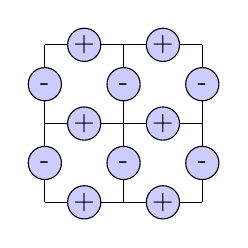
\begin{tikzpicture}[
            baseline={([yshift=-0.5ex]current bounding box.center)},
            site/.style={circle,draw,fill=blue!20,minimum size=#1,
                inner sep=0pt, outer sep=0pt},
            site/.default=12pt
        ]
        \draw (0, 0) -- node[site] {-}  (0, 1);
        \draw (0, 1) -- node[site] {-}  (0, 2);
        \draw (1, 0) -- node[site] {-}  (1, 1);
        \draw (1, 1) -- node[site] {-}  (1, 2);
        \draw (2, 0) -- node[site] {-}  (2, 1);
        \draw (2, 1) -- node[site] {-}  (2, 2);
        \draw (0, 0) -- node[site] {+}  (1, 0);
        \draw (0, 1) -- node[site] {+}  (1, 1);
        \draw (0, 2) -- node[site] {+}  (1, 2);
        \draw (1, 0) -- node[site] {+}  (2, 0);
        \draw (1, 1) -- node[site] {+}  (2, 1);
        \draw (1, 2) -- node[site] {+}  (2, 2);
    \end{tikzpicture}\quad = \quad
    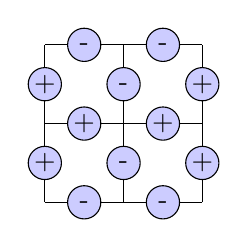
\begin{tikzpicture}[
            baseline={([yshift=-0.5ex]current bounding box.center)},
            site/.style={circle,draw,fill=blue!20,minimum size=#1,
                inner sep=0pt, outer sep=0pt},
            site/.default=12pt
        ]
        \draw (0, 0) -- node[site] {+}  (0, 1);
        \draw (0, 1) -- node[site] {+}  (0, 2);
        \draw (1, 0) -- node[site] {-}  (1, 1);
        \draw (1, 1) -- node[site] {-}  (1, 2);
        \draw (2, 0) -- node[site] {+}  (2, 1);
        \draw (2, 1) -- node[site] {+}  (2, 2);
        \draw (0, 0) -- node[site] {-}  (1, 0);
        \draw (0, 1) -- node[site] {+}  (1, 1);
        \draw (0, 2) -- node[site] {-}  (1, 2);
        \draw (1, 0) -- node[site] {-}  (2, 0);
        \draw (1, 1) -- node[site] {+}  (2, 1);
        \draw (1, 2) -- node[site] {-}  (2, 2);
    \end{tikzpicture} \quad = \quad
    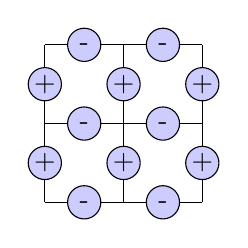
\begin{tikzpicture}[
            baseline={([yshift=-0.5ex]current bounding box.center)},
            site/.style={circle,draw,fill=blue!20,minimum size=#1,
                inner sep=0pt, outer sep=0pt},
            site/.default=12pt
        ]
        \draw (0, 0) -- node[site] {+}  (0, 1);
        \draw (0, 1) -- node[site] {+}  (0, 2);
        \draw (1, 0) -- node[site] {+}  (1, 1);
        \draw (1, 1) -- node[site] {+}  (1, 2);
        \draw (2, 0) -- node[site] {+}  (2, 1);
        \draw (2, 1) -- node[site] {+}  (2, 2);
        \draw (0, 0) -- node[site] {-}  (1, 0);
        \draw (0, 1) -- node[site] {-}  (1, 1);
        \draw (0, 2) -- node[site] {-}  (1, 2);
        \draw (1, 0) -- node[site] {-}  (2, 0);
        \draw (1, 1) -- node[site] {-}  (2, 1);
        \draw (1, 2) -- node[site] {-}  (2, 2);
    \end{tikzpicture} \quad = \quad $\cdots$
    \caption{gauge freedom in the $2$-cell case (plaquette),
    $H_1$ is the same for these configurations.
    2nd configuration is obtained by flipping all
    spins attached to center vertex, 3rd configuration is obtained
    by flipping all spins attached all vertices.}\label{fig:2-cell-gauge}
\end{figure}

Similarly, if $p=2, d=3$, on the faces of a cube, the 4 faces attached to the same
edge can flip their spins. Thus we have a free spin on each edge of number $N_1$.
However, this over-counts because when flipping all the effective spin on the edges that
attached to the same vertex corresponding to the same face spins. Thus the total
number of free spins should be $N_1 - N_0$.

Thus following this derivation, and generalize the above conclusion.
We know, the free spins at $p$-cell is flipping
all spins of $p$-cell that attached to $p-1$-cell,
and the free spins for general $p$ can be obtained by counting
the free spins of $p-1$ case. Thus we have

$$
\begin{aligned}
    N_{free} &= N_{p-1} - (N_{p-2} - (N_{p-3} - \cdots (N_1 - N_0)))\\
    &=N_{p-1} - N_{p-2} + N_{p-3} - \cdots N_1 \pm N_0\\
\end{aligned}
$$

thus the ground state degeneracy is $2^{N_{p-1} - N_{p-2} + N_{p-3} - \cdots N_1 \pm N_0}$
for hypercubic lattice with no defects (the defects will create an $O(1)$ correction to
the degeneracy).

This gives the residual entropy of the ground state,

$$
S/N = \frac{N_{p-1} - N_{p-2} + N_{p-3} - \cdots N_1 \pm N_0}{N_0} log(2)
$$

for $p=2,d=3$ case, we have $N_1 = 3N_0$, thus $S/N = 2log(2)$

\begin{figure}[h]
    \centering
    \includestandalone{images/cube}
\end{figure}

However, the above derivation can be much simpler, which is two sentence in the original
self-correcting memory paper\cite{hastings2014self}. It is actually the Euler characteristic
of the cell chain complex. Or the Betti number as the rank of the $n$-th singular homology
group\cite{wiki-euler-characteristic,algebra-topology-sjer}.

% Now I will discuss some formal definitions of above concepts in
% terms of homology based on this nice PhD thesis from Rene about
% concepts for scientific computing and programming languages\cite{topology1977rene}.
% We will see that the lattices we used in physics shares the same algebraic property\cite{wiki-lattice}
% with many other things, such as type system in programming language. And they can all
% visualize as a lattice-like diagram under Hasse diagram.

% \begin{definition}
%     (Topology) A topological space $(\mathcal{X}, \mathcal{T})$ consists of a set $\mathcal{X}$ and set $\mathcal{T}$
%     of subsets, called open sets, of $\mathcal{X}$ such that:
%     \begin{itemize}
%         \item $\emptyset \in \mathcal{T}$ and $\mathcal{X} \in \mathcal{T}$
%         \item a finite intersection of members of $\mathcal{T}$ is in $\mathcal{T}$
%         \item an arbitrary union of members of $\mathcal{T}$ is in $\mathcal{T}$
%     \end{itemize}
% \end{definition}

% In our 2-dim case (square lattice), the $N_0$ vertices, $N_1$ edges, and $N_2$ plaquettes forms a topology. This
% is because: a) $\emptyset$ and all vertices of the lattice belongs to $\mathcal{T}$
% b) any finite union of vertex sets creates an edge set. And any finite union of
% edge set creates a plaquette set. c) any union between the above is in $\mathcal{T}$

% Another example of tree elements from the thesis is a basic set $\mathcal{X} = \{a, b, c\}$, and the corresponding
% topology of it is
% $$
% \begin{aligned}
%     (\mathcal{X}, \mathcal{T}) = \set{
%         \emptyset, \set{a}, \set{b}, \set{c},
%         \set{a,b}, \set{a,c}, \set{b,c},
%         \set{a,b,c}
%     }
% \end{aligned}
% $$

% \begin{definition}
%     (Hausdorff spaces) The topological space $(\mathcal{X}, \mathcal{T})$ is said to be Hausdorff if,
%     given $x, y\in X$ with $x \neq y$, there exists open sets $U_1, U_2$ such that $x\in U_1, y\in U_2$ and
%     $U_1\cap U_2 = \emptyset$.
% \end{definition}

% \begin{definition}
%     (Open Cell) A subset $c \subset X$ of a Hausdorff space $X$ is an open cell if it is
%     homeomorphic to the interior of an open $p$-dim ball $\mathbb{D}^p = \{x \in \mathbb{R}^p: \abs{x} < 1\}$.
% \end{definition}

% Collections of cells form larger structures, so-called complexes which are identified by the cell with the highest
% dimension, e.g. a $p$-dimensional space contains $p$-cells.

% \begin{definition}
%     (Cover) A cover of a set $X$ is a set of nonempty subsets of $X$ whose union is $X$.
% \end{definition}

% A cover is an open cover if it is contained in the topology.

% \section{Quon representation of the partition function}

% $$
% \begin{aligned}
%     A &= \begin{pmatrix}
%         e^{\beta} & e^{-\beta}\\
%         e^{-\beta} & e^{\beta}\\
%     \end{pmatrix}\\
%     \det{A - \lambda I} &= 0\\
%     \det{\begin{pmatrix}
%         e^{\beta} - \lambda & e^{-\beta}\\
%         e^{-\beta} & e^{\beta} - \lambda
%     \end{pmatrix}} &= 0\\
%     (e^{\beta}-\lambda)^2 &= e^{-2\beta}\\
%     e^{\beta} - \lambda &= \pm e^{-\beta}\\
%     \lambda &= e^{\beta} \pm e^{-\beta}\\
%     D &= \begin{pmatrix}
%         e^{\beta} + e^{-\beta} & 0\\
%         0 & e^{\beta} - e^{-\beta}
%     \end{pmatrix}
%     (A - \lambda I)x &= 0\\
%     \begin{pmatrix}
%         -1 & 1\\
%         1 & -1
%     \end{pmatrix} x = 0\quad &\text{or} \quad \begin{pmatrix}
%         1 & 1\\
%         1 & 1
%     \end{pmatrix}x = 0\\
%     x = \begin{pmatrix}
%         1\\
%         1
%     \end{pmatrix} \quad &\text{or} \begin{pmatrix}
%         1\\
%         -1
%     \end{pmatrix}
% \end{aligned}
% $$

% thus 

% $$
% \begin{pmatrix}
%     e^{\beta} & e^{-\beta}\\
%     e^{-\beta} & e^{\beta}\\
% \end{pmatrix} = H \begin{pmatrix}
%     e^{\beta} + e^{-\beta} & 0\\
%     0 & e^{\beta} - e^{-\beta}
% \end{pmatrix} H^T
% $$

\bibliographystyle{plain}
\bibliography{ref}

\end{document}